\documentclass[a4paper,11pt]{report}
\usepackage{chuan_math_gkt}
\usetikzlibrary{angles,quotes,intersections,patterns,decorations.pathreplacing}
\chuanexamsetup

\begin{document}
\examfontsize

\examsecret{绝密$\bigstar$启用前}

\examtitle{2020年普通高等学校招生全国统一考试（北京卷）}{数\quad 学}

\noticetitle
\begin{examnotice}
\item 答卷前，考生务必将自己的姓名、准考证号填写在答题卡上。
\item 回答选择题时，选出每小题的答案后，用铅笔把答题卡上对应题目的答案标号涂黑。如需改动，用橡皮擦干净后，再选涂其他答案标号。回答非选择题时，将答案写在答题卡上。写在本试卷上无效。
\item 考试结束后，将本试卷和答题卡一并交回。
\end{examnotice}


\examsection{一、选择题：本题共10小题，每小题4分，共40分。在每小题给出的四个选项中，只有一项是符合题目要求的。}
\begin{examquestions}
\item 已知集合 $A=\{-1,0,1,2\}$，$B=\{x\mid 0<x<3\}$，则 $A\cap B=$
\fourchoices{$\{-1,0,1\}$}{$\{0,1\}$}{$\{-1,1,2\}$}{$\{1,2\}$}
\item 在复平面内，复数 $z$ 对应的点的坐标是 $(1,2)$，则 $\mathrm{i}z=$
\fourchoices{$1+2\mathrm{i}$}{$-2+\mathrm{i}$}{$1-2\mathrm{i}$}{$-2-\mathrm{i}$}
\item 在 $(\sqrt{x}-2)^5$ 的展开式中，$x^2$ 的系数为
\fourchoices{$-5$}{$5$}{$-10$}{$10$}
\item 某三棱柱的底面为正三角形，其三视图如图所示，该三棱柱的表面积为
\fourchoices{$6+\sqrt3$}{$6+2\sqrt3$}{$12+\sqrt3$}{$12+2\sqrt3$}
\begin{tightcenter}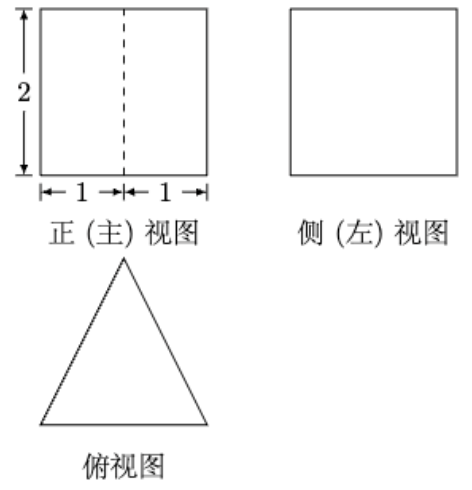
\includegraphics[width=5.3cm]{figures/2020_bj_q4.png}\end{tightcenter}
\item 已知半径为 $1$ 的圆经过点 $(3,4)$，则其圆心到原点的距离的最小值为
\fourchoices{$4$}{$5$}{$6$}{$7$}
\item 已知函数 $f(x)=2^x-x-1$，则不等式 $f(x)>0$ 的解集是
\twochoices{$(-1,1)$}{$(-\infty,-1)\cup(1,+\infty)$}{$(0,1)$}{$(-\infty,0)\cup(1,+\infty)$}
\item 设抛物线的顶点为 $O$，焦点为 $F$，准线为 $l$，$P$ 是抛物线上异于 $O$ 的一点，过 $P$ 作 $PQ\perp l$ 于 $Q$，则线段 $FQ$ 的垂直平分线
\fourchoices{经过点 $O$}{经过点 $P$}{平行于直线 $OP$}{垂直于直线 $OP$}
\item 在等差数列 $\{a_n\}$ 中，$a_1=-9$，$a_5=-1$，记 $T_n=a_1a_2\cdots a_n$，则数列 $\{T_n\}$
\twochoices{有最大项，有最小项}{有最大项，无最小项}{无最大项，有最小项}{无最大项，无最小项}
\item 已知 $\alpha,\beta\in\mathbb R$，则“存在 $k\in\mathbb Z$，使得 $\alpha=k\pi+(-1)^k\beta$”是“$\sin\alpha=\sin\beta$”的
\twochoices{充分而不必要条件}{必要而不充分条件}{充分必要条件}{既不充分也不必要条件}
\item $2020$年$3$月$14$日是全球首个国际圆周率日（$\pi$ Day）. 历史上，求圆周率 $\pi$ 的方法有多种，与中国传统数学中的“割圆术”相似，数学家阿尔·卡西的方法是：当正整数 $n$ 充分大时，计算单位圆的内接正 $6n$ 边形的周长和外切正 $6n$ 边形的周长，将它们的算术平均数作为 $2\pi$ 的近似值. 按照阿尔·卡西的方法，$\pi$ 的近似值的表达式是
\twochoices{\tallchoice{$3n\left(\sin\dfrac{30^\circ}{n}+\tan\dfrac{30^\circ}{n}\right)$}}{\tallchoice{$6n\left(\sin\dfrac{30^\circ}{n}+\tan\dfrac{30^\circ}{n}\right)$}}{\tallchoice{$3n\left(\sin\dfrac{60^\circ}{n}+\tan\dfrac{60^\circ}{n}\right)$}}{\tallchoice{$6n\left(\sin\dfrac{60^\circ}{n}+\tan\dfrac{60^\circ}{n}\right)$}}
\end{examquestions}

\examsection{二、填空题：本题共5小题，每小题5分，共25分。}
\begin{examquestions}[start=11]
\item 函数 $f(x)=\ln x+\dfrac{1}{x+1}$ 的定义域是\blank.
\item 已知双曲线 $C:\dfrac{x^2}{6}-\dfrac{y^2}{3}=1$，则 $C$ 的右焦点的坐标为\blank；$C$ 的焦点到其渐近线的距离是\blank.
\item 已知正方形 $ABCD$ 的边长为 $2$，点 $P$ 满足 $\vec{AP}=\dfrac12(\vec{AB}+\vec{AC})$，则 $|\vec{PD}|=$\blank；$\vec{PB}\cdot\vec{PD}=$\blank.
\item 若函数 $f(x)=\sin(x+\varphi)+\cos x$ 的最大值为 $2$，则常数 $\varphi$ 的一个取值为\blank.
\newpage
\item 为满足人民对美好生活的向往，环保部门要求企业加强污水治理，排放未达标的企业要限期整改，设企业的污水排放量 $W$ 与时间 $t$ 的关系为 $W=f(t)$，用 $\dfrac{f(t_1)-f(t_2)}{t_2-t_1}$ 的大小评价在 $[t_1,t_2]$ 这段时间内企业污水治理能力的强弱. 已知整改期内，甲、乙两企业的污水排放量与时间的关系如下图所示.
\begin{tightcenter}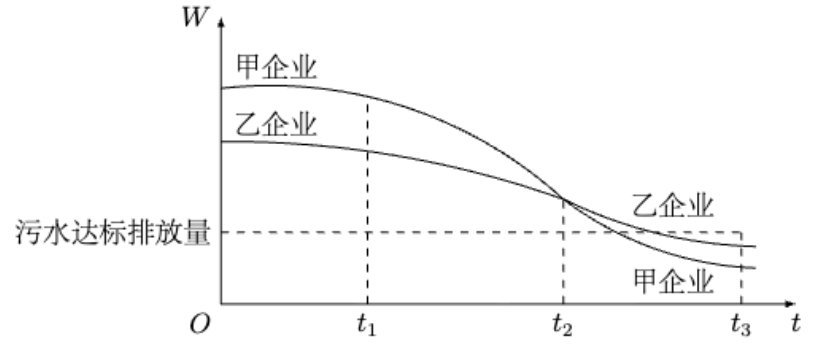
\includegraphics[width=9.5cm]{figures/2020_bj_q15.png}\end{tightcenter}
给出下列四个结论：①在 $[t_1,t_2]$ 这段时间内，甲企业的污水治理能力比乙企业强；②在 $t_2$ 时刻，甲企业的污水治理能力比乙企业强；③在 $t_3$ 时刻，甲、乙两企业的污水排放都已达标；④甲企业在 $[t_1,t_2]$，$[t_2,t_3]$，$[t_3,t_4]$ 这三段时间中，在 $[t_2,t_3]$ 的污水治理能力最强. 其中所有正确结论的序号是\blank.
\end{examquestions}

\examsection{三、解答题：本题共6小题，共85分。解答应写出文字说明、证明过程或演算步骤。}
\begin{examanswers}[start=16]
\item（13分）

如图，在正方体 $ABCD-A_1B_1C_1D_1$ 中，$E$ 为 $BB_1$ 的中点.

\noindent\begin{minipage}[t]{0.64\linewidth}
（1）求证：$BC_1\parallel$ 平面 $AD_1E$；

（2）求直线 $AA_1$ 与平面 $AD_1E$ 所成角的正弦值.
\end{minipage}\hfill
\begin{minipage}[t]{0.30\linewidth}
\vspace{-1.0em}\centering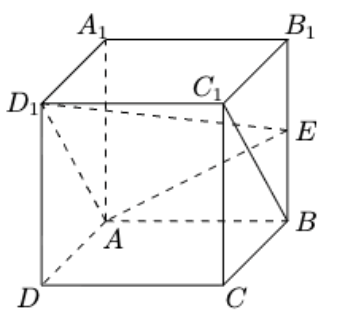
\includegraphics[width=\linewidth]{figures/2020_bj_q16.png}
\end{minipage}
\item（13分）

在 $\triangle ABC$ 中，$a+b=11$，再从条件①、条件②这两个条件中选择一个作为已知，求：

（1）$a$ 的值；

（2）$\sin C$ 和 $\triangle ABC$ 的面积.

条件①：$c=7$，$\cos A=-\dfrac17$；

条件②：$\cos A=\dfrac18$，$\cos B=\dfrac9{16}$.
\item（14分）

某校为举办甲、乙两项不同活动，分别设计了相应的活动方案：方案一、方案二. 为了了解该校学生对活动方案是否支持，对学生进行简单随机抽样，获得数据如下表：
\begin{tightcenter}
    {\renewcommand{\arraystretch}{0.9}
\begin{tabular}{c|cc|cc}
\hline
 & \multicolumn{2}{c|}{男生} & \multicolumn{2}{c}{女生}\\
 & 支持 & 不支持 & 支持 & 不支持\\ \hline
方案一 & 200人 & 400人 & 300人 & 100人\\
方案二 & 350人 & 250人 & 150人 & 250人\\ \hline
\end{tabular}}
\end{tightcenter}
假设所有学生对活动方案是否支持相互独立.

（1）分别估计该校男生支持方案一的概率、该校女生支持方案一的概率；

（2）从该校全体男生中随机抽取 $2$ 人，全体女生中随机抽取 $1$ 人，估计这 $3$ 人中恰有 $2$ 人支持方案一的概率；

（3）将该校学生支持方案二的概率估计值记为 $p_0$. 假设该校一年级有 $500$ 名男生和 $300$ 名女生，除一年级外其他年级学生支持方案二的概率估计值记为 $p_1$，试比较 $p_0$ 与 $p_1$ 的大小.（结论不要求证明）
\vspace{-2.4em}
\item（15分）

已知函数 $f(x)=12-x^2$.

（1）求曲线 $y=f(x)$ 的斜率等于 $-2$ 的切线方程；

（2）设曲线 $y=f(x)$ 在点 $(t,f(t))$ 处的切线与坐标轴围成的三角形的面积为 $S(t)$，求 $S(t)$ 的最小值.
\vspace{-2.4em}
\item（15分）

已知椭圆 $C:\dfrac{x^2}{a^2}+\dfrac{y^2}{b^2}=1$ 过点 $A(-2,-1)$，且 $a=2b$.

（1）求椭圆 $C$ 的方程；

（2）过点 $B(-4,0)$ 的直线 $l$ 交椭圆 $C$ 于点 $M$，$N$，直线 $MA$，$NA$ 分别交直线 $x=-4$ 于点 $P$，$Q$，求 $\dfrac{|PB|}{|BQ|}$ 的值.

\vspace{-2.4em}
\item（15分）

已知 $\{a_n\}$ 是无穷数列，给出两个性质：①对于 $\{a_n\}$ 中任意两项 $a_i,a_j(i>j)$，在 $\{a_n\}$ 中都存在一项 $a_m$，使得 $\dfrac{a_i^2}{a_j}=a_m$；②对于 $\{a_n\}$ 中任意一项 $a_n(n\geq3)$，在 $\{a_n\}$ 中都存在两项 $a_k,a_l(k>l)$，使得 $a_n=\dfrac{a_k^2}{a_l}$.

（1）若 $a_n=n(n=1,2,\cdots)$，判断数列 $\{a_n\}$ 是否满足性质①，说明理由；

（2）若 $a_n=2^{n-1}(n=1,2,\cdots)$，判断数列 $\{a_n\}$ 是否同时满足性质①、②，说明理由；

（3）若 $\{a_n\}$ 是递增数列，且同时满足性质①和性质②，证明：$\{a_n\}$ 为等比数列.
\end{examanswers}

\end{document}
